\documentclass[tikz,border=3.14mm]{standalone}

\begin{document}

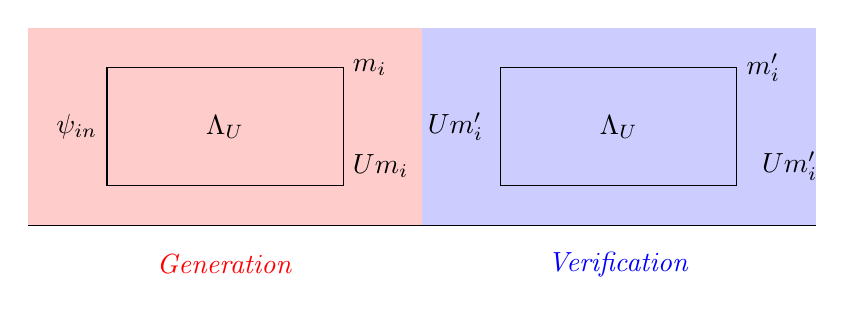
\begin{tikzpicture}
    % Draw the big box
    \draw (0,0) rectangle (10,2.5);
    
    % Draw the left box (Generation)
    \fill[red!20] (0,0) rectangle (5,2.5);
    \node at (2.5,-0.5) {\textcolor{red}{\emph{Generation}}};
    
    % Draw the right box (Verification)
    \fill[blue!20] (5,0) rectangle (10,2.5);
    \node at (7.5,-0.5) {\textcolor{blue}{\emph{Verification}}};
    
    % Generation Box
    \draw (1,0.5) rectangle (4,2);
    \node at (2.5,1.25) {$\Lambda_U$};
    \node[left] at (1,1.25) {$\ket{\psi_{in}}$};
    \node[right] at (4,2) {$m_i$};
    \node[right] at (4,0.75) {$U\ket{m_i}$};
    
    % Verification Box
    \draw (6,0.5) rectangle (9,2);
    \node at (7.5,1.25) {$\Lambda_U$};
    \node[left] at (6,1.25) {$\;\;U\ket{m_i'}\;$}; % adjusted for alignment
    \node[right] at (9,2) {$m'_i$};
    \node[right] at (9,0.75) {$\;\;U\ket{m'_i}\;$}; % adjusted for alignment
\end{tikzpicture}

\end{document}